%!TEX root = ../thesis.tex
%*******************************************************************************
%******************************* Introduction **********************************
%*******************************************************************************

\ifsetDraft
\else
    \cleartoevenpage
    \backgroundsetup{
        scale=1,
        color=black,
        opacity=1,
        placement=top,
        angle=0,
        contents={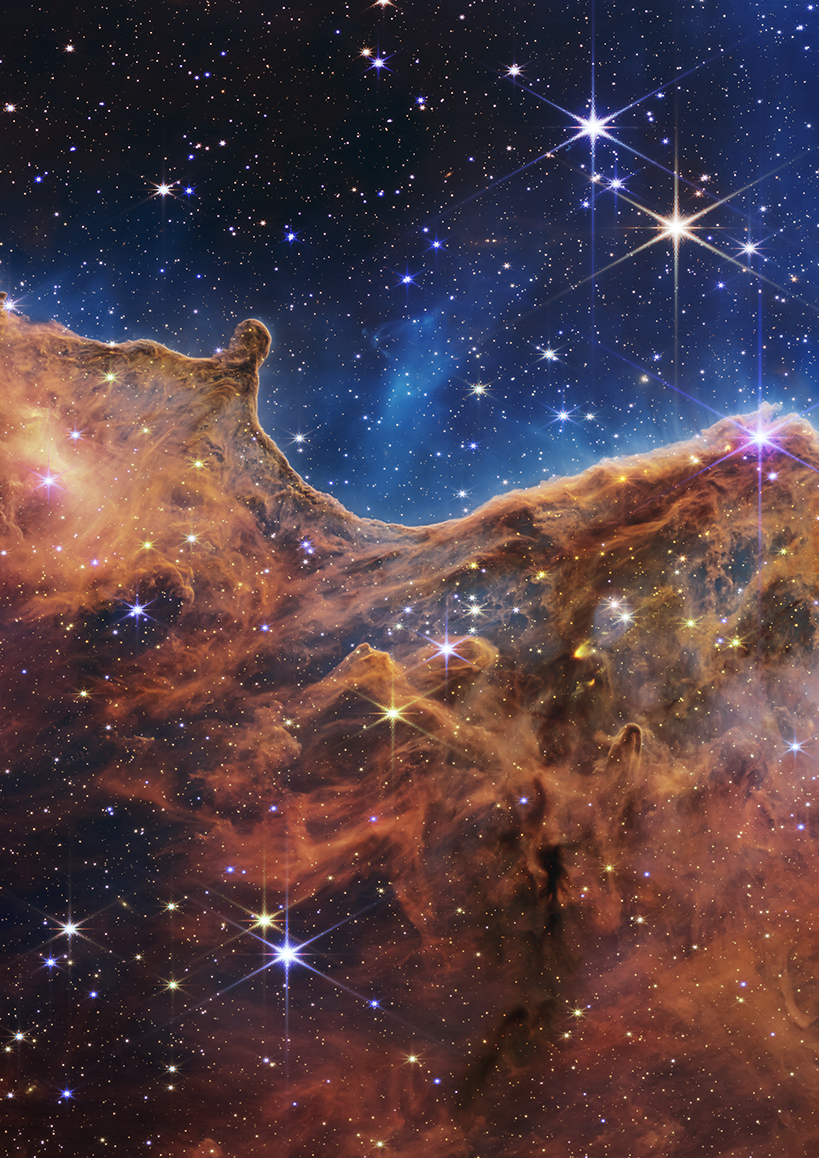
\includegraphics[width=\paperwidth]{Images/Carina_nebula1}}
    }
    \BgThispage
    
    \fancyfoot[C]{\color{white}\thepage}
    \fancyfoot[L]{\vspace{3.5ex}\tiny\textcolor{white}{Credit: NASA, ESA, CSA, STScI}}
    \clearpage
    \newpage
    
    \renewcommand{\CurrentTitleColor}{\color{white}}
\fi

\chapter{Conclusions}
\label{ch:Conclusions}

\ifsetDraft
\else
    \renewcommand{\CurrentTitleColor}{\color{black}}
    
    \backgroundsetup{
        scale=1,
        color=black,
        opacity=1,
        placement=top,
        angle=0,
        contents={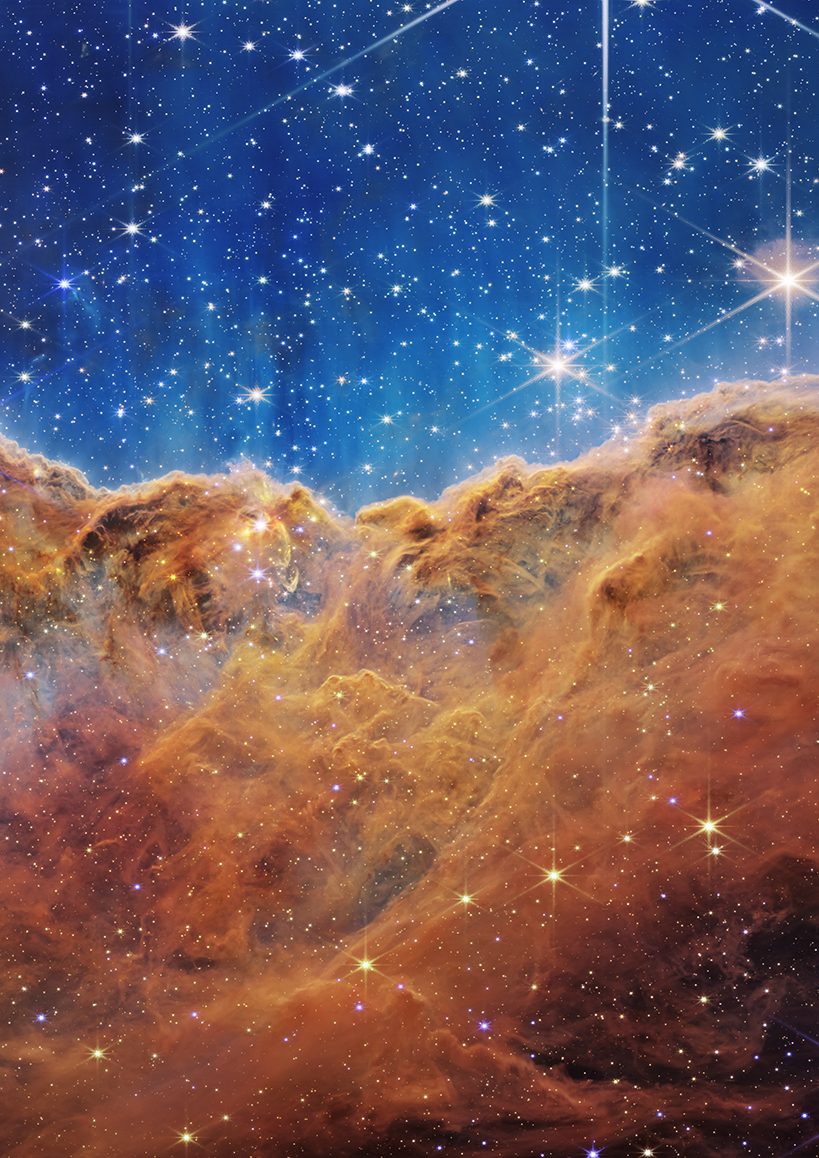
\includegraphics[width=\paperwidth]{Images/Carina_nebula2}}
    }
    \BgThispage
    
    \fancyhf{}
    \fancyfoot[C]{\color{white}\thepage}
    \newpage
    \setFancyHdr
\fi

\section{Conclusions}

\lettrine{I}{n the previous chapters}, we have discussed the properties of star-forming galaxies and the intergalactic medium in the early Universe. 

\section{Outlook}

